\documentclass[tikz,border=5pt]{standalone}
\usepackage{tikz}
\usepackage{amsmath,amssymb}
\usetikzlibrary{positioning,arrows.meta,fit,calc,backgrounds}

%% ── Palette ──────────────────────────────────────────────────────────────────
\definecolor{corecol}{RGB}{41,98,178}
\definecolor{corelite}{RGB}{218,228,252}
\definecolor{arcol}{RGB}{190,75,20}
\definecolor{disccol}{RGB}{110,35,160}
\definecolor{elfcol}{RGB}{15,120,85}

\begin{document}
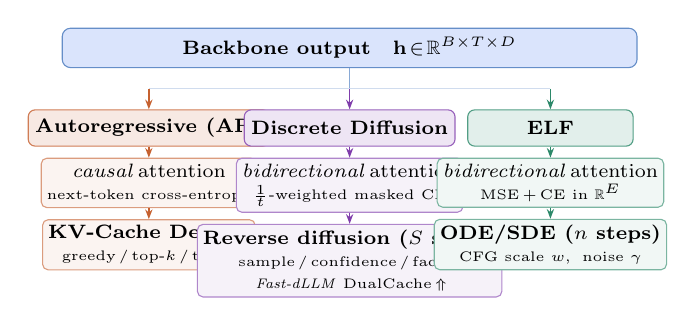
\begin{tikzpicture}[
  every node/.style={font=\scriptsize},
  %% coloured column block  \node[col=arcol]{...}
  col/.style={
    draw=#1!72, fill=#1!12,
    rounded corners=2.5pt,
    minimum width=2.10cm, minimum height=0.46cm,
    align=center, inner sep=2.5pt
  },
  col/.default=corecol,
  %% smaller detail block inside a column
  det/.style={
    draw=#1!55, fill=#1!6,
    rounded corners=2pt,
    minimum width=2.10cm, minimum height=0.44cm,
    align=center, inner sep=2pt
  },
  det/.default=corecol,
  %% coloured arrows
  arr/.style={-{Stealth[length=3.5pt,width=2.6pt]}, semithick, color=#1!88},
  arr/.default=corecol,
]

%%── Shared backbone output (full-width header) ───────────────────────────────
\node[draw=corecol!72, fill=corelite,
      rounded corners=3pt,
      minimum width=7.30cm, minimum height=0.50cm,
      align=center, inner sep=2.5pt] (h)
  {\textbf{Backbone output}\quad
   $\mathbf{h}\!\in\!\mathbb{R}^{B\times T\times D}$};

%%── Three-way split: short stem + horizontal bus + drops ─────────────────────
\coordinate (sp) at ($(h.south)+(0,-0.26cm)$);
\draw[-,semithick,corecol!55] (h.south) -- (sp);
\draw[-,thin,corecol!22]
  ($(sp)+(-2.55cm,0)$) -- ($(sp)+(2.55cm,0)$);

%%══════════════════════════════════════════════════════════════════════════════
%%  AR  (left column)
%%══════════════════════════════════════════════════════════════════════════════
\node[col=arcol] (ar0)
  at ($(h.south)+(-2.55cm,-0.76cm)$)
  {\textbf{Autoregressive (AR)}};

\node[det=arcol, below=0.14cm of ar0] (ar1)
  {\textit{causal}\,attention\\
   {\tiny next-token cross-entropy}};

\node[det=arcol, below=0.14cm of ar1] (ar2)
  {\textbf{KV-Cache Decode}\\
   {\tiny greedy\,/\,top-$k$\,/\,top-$p$}};

%%══════════════════════════════════════════════════════════════════════════════
%%  DISCRETE DIFFUSION  (centre column)
%%══════════════════════════════════════════════════════════════════════════════
\node[col=disccol] (disc0)
  at ($(h.south)+(0,-0.76cm)$)
  {\textbf{Discrete Diffusion}};

\node[det=disccol, below=0.14cm of disc0] (disc1)
  {\textit{bidirectional}\,attention\\
   {\tiny $\tfrac{1}{t}$-weighted masked CE}};

\node[det=disccol, below=0.14cm of disc1] (disc2)
  {\textbf{Reverse diffusion ($S$ steps)}\\
   {\tiny sample\,/\,confidence\,/\,factor}\\
   {\tiny \textit{Fast-dLLM} DualCache\,$\Uparrow\!$}};

%%══════════════════════════════════════════════════════════════════════════════
%%  ELF  (right column)
%%══════════════════════════════════════════════════════════════════════════════
\node[col=elfcol] (elf0)
  at ($(h.south)+(2.55cm,-0.76cm)$)
  {\textbf{ELF}};

\node[det=elfcol, below=0.14cm of elf0] (elf1)
  {\textit{bidirectional}\,attention\\
   {\tiny MSE\,+\,CE in $\mathbb{R}^{E}$}};

\node[det=elfcol, below=0.14cm of elf1] (elf2)
  {\textbf{ODE/SDE ($n$ steps)}\\
   {\tiny CFG scale $w$,\; noise $\gamma$}};

%%── Arrows: bus drop → column headers ───────────────────────────────────────
\draw[arr=arcol]   ($(sp)+(-2.55cm,0)$) -- (ar0.north);
\draw[arr=disccol] (sp)                  -- (disc0.north);
\draw[arr=elfcol]  ($(sp)+(2.55cm,0)$)  -- (elf0.north);

%%── Within-column arrows ─────────────────────────────────────────────────────
\draw[arr=arcol]   (ar0)   -- (ar1);
\draw[arr=arcol]   (ar1)   -- (ar2);
\draw[arr=disccol] (disc0) -- (disc1);
\draw[arr=disccol] (disc1) -- (disc2);
\draw[arr=elfcol]  (elf0)  -- (elf1);
\draw[arr=elfcol]  (elf1)  -- (elf2);

\end{tikzpicture}
\end{document}
